\section[Maven]{Maven}
\subsection[]{Introduction}
\begin{frame}
\frametitle{Building java applications}
\begin{itemize}
	\item Motivation aka \emph{Why should we care, let's have bash script with bunch of javac commands}
	\item Brief look into history
		\begin{itemize}
		\item Make % 1977
		\item Ant (with Ivy) %XML - 2000
		\item Maven %XML  - 2005
		\item Gradle %DSL based on Groovy (used by google to build Android), less boilerplate - 2012
		\end{itemize}
\end{itemize}
\end{frame}

% Ant
%    -  XML, procedural, scripting tool, originally intended to replace make
%    - nothing is standardized (clean vs clear)
%    - need to explicitely do everything
%    - easier to learn than maven (but is really just a scripting tool)

\begin{frame}
\frametitle{Build tools - history overview}
	\begin{center}
		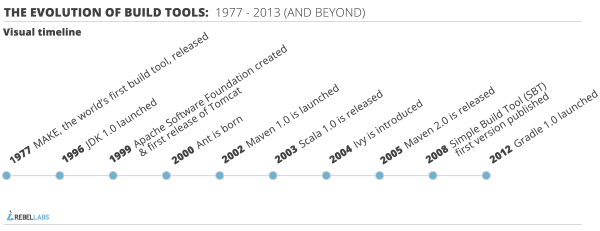
\includegraphics[width=\textwidth,height=0.385\textwidth]{build-tools-history.png}
	\end{center}
\end{frame}

\begin{frame}
\frametitle{Build tools - popularity}
	\begin{center}
		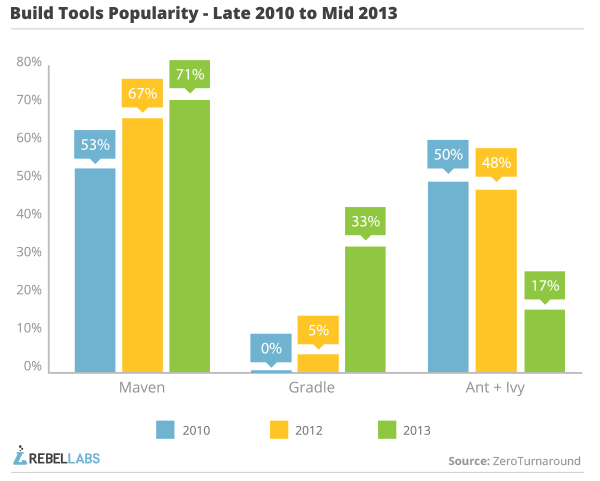
\includegraphics[width=0.8\textwidth,height=0.64\textwidth]{build-tools-popularity.png}
	\end{center}
\end{frame}

\begin{frame}
\frametitle{Desired properties of quality build tool}
\begin{itemize}
	\item How steep is learning curve
	\item Time required for build
	\item Complexity of build script (creation, maintenance)
	\item Extensibility and flexibility (plugins)
	\item Build environment consistency
	\item Extra features (docs, deployment, etc...)
	\item Integration with developer tools (IDEs, CI servers,...)
\end{itemize}
\end{frame}



\begin{frame}
\frametitle{Maven - Best practices}
\begin{itemize}
\item something
\end{itemize}
\end{frame}




\subsection[]{Maven - Demo}
\begin{frame}
\frametitle{Maven - Demo}
\end{frame}








